\documentclass[a4paper,showframe,11pt]{report}\usepackage[]{graphicx}\usepackage[]{color}
%% maxwidth is the original width if it is less than linewidth
%% otherwise use linewidth (to make sure the graphics do not exceed the margin)
\makeatletter
\def\maxwidth{ %
  \ifdim\Gin@nat@width>\linewidth
    \linewidth
  \else
    \Gin@nat@width
  \fi
}
\makeatother

\definecolor{fgcolor}{rgb}{0.196, 0.196, 0.196}
\newcommand{\hlnum}[1]{\textcolor[rgb]{0.063,0.58,0.627}{#1}}%
\newcommand{\hlstr}[1]{\textcolor[rgb]{0.063,0.58,0.627}{#1}}%
\newcommand{\hlcom}[1]{\textcolor[rgb]{0.588,0.588,0.588}{#1}}%
\newcommand{\hlopt}[1]{\textcolor[rgb]{0.196,0.196,0.196}{#1}}%
\newcommand{\hlstd}[1]{\textcolor[rgb]{0.196,0.196,0.196}{#1}}%
\newcommand{\hlkwa}[1]{\textcolor[rgb]{0.231,0.416,0.784}{#1}}%
\newcommand{\hlkwb}[1]{\textcolor[rgb]{0.627,0,0.314}{#1}}%
\newcommand{\hlkwc}[1]{\textcolor[rgb]{0,0.631,0.314}{#1}}%
\newcommand{\hlkwd}[1]{\textcolor[rgb]{0.78,0.227,0.412}{#1}}%
\let\hlipl\hlkwb

\usepackage{framed}
\makeatletter
\newenvironment{kframe}{%
 \def\at@end@of@kframe{}%
 \ifinner\ifhmode%
  \def\at@end@of@kframe{\end{minipage}}%
  \begin{minipage}{\columnwidth}%
 \fi\fi%
 \def\FrameCommand##1{\hskip\@totalleftmargin \hskip-\fboxsep
 \colorbox{shadecolor}{##1}\hskip-\fboxsep
     % There is no \\@totalrightmargin, so:
     \hskip-\linewidth \hskip-\@totalleftmargin \hskip\columnwidth}%
 \MakeFramed {\advance\hsize-\width
   \@totalleftmargin\z@ \linewidth\hsize
   \@setminipage}}%
 {\par\unskip\endMakeFramed%
 \at@end@of@kframe}
\makeatother

\definecolor{shadecolor}{rgb}{.97, .97, .97}
\definecolor{messagecolor}{rgb}{0, 0, 0}
\definecolor{warningcolor}{rgb}{1, 0, 1}
\definecolor{errorcolor}{rgb}{1, 0, 0}
\newenvironment{knitrout}{}{} % an empty environment to be redefined in TeX

\usepackage{alltt}
\usepackage{standalone}
\standalonetrue
\ifstandalone
  \usepackage{../../haziq_thesis}
  \usepackage{../../haziq_maths}
  \usepackage{../../haziq_glossary}
  \addbibresource{../../bib/haziq.bib}
  \externaldocument{../01/.texpadtmp/introduction}
\fi





\IfFileExists{upquote.sty}{\usepackage{upquote}}{}
\begin{document}

Machine learning tools are being used in the field of medicine as a means to aid medical diagnosis of diseases. In this example, factors determining the presence or absence of heart diseses is studied. Traditionally, cardiologists may look at patients' cardiac activity (ECG data) to reach a diagnosis. This of course remains the so-called ``gold standard'' method of obtaining a diagnosis. The study by Guvenir et. al. aimed to predict cardiac abnormalities by way of machine learning and minimise the difference between the gold standard and computer-based classifications. This data set is made publicly available at [...]. It contains a myriad of ECG readings and other patient attributes such as age, height, and weight. Altogether there are 451 observations and 279 predictors. We excluded nominal covariates, leaving us with 194 continuous predictors, which we then standardised so that we can use a single-scale I-probit model. In the original data set, there are 13 distinct classes of cardiac arrhythmia. We had combined all of these to form a single class, thus reducing the problem to a binary classification task (normal vs. arrhythmia).

Fitting an I-probit model on the full data set takes about 2.5 seconds only, with convergence reached in at most 15 iterations.
However, we do find that the training error rates are much better if the model was not allowed to reach full convergence (i.e., stopped early at five iterations, say)
\hltodo{Why is this? Need to look at a plot of marginal likelihood.}.
It is believed that local optima gives better predictive performance, rather than at the global maxima of the (approximate) likelihood.

Figure \ref{fig:cardiac.mod.full.plot}(a) plots the variational lower bound value over time and iterations for the cardiac arrhythmia data set. As expected, the lower bound value increases over time until a convergence criterion is reached. In Figure \ref{fig:cardiac.mod.full.plot}(b), the training error rate and the Brier score is plotted against time. What we see is that the training error rate worsens over time as the lower bound value reaches its maximum value. There is some reason to terminate the variational algorithm early - while compromising on the lower bound value, we hope to obtain parameter values which give good predictive performance.


\begin{knitrout}
\definecolor{shadecolor}{rgb}{1, 1, 1}\color{fgcolor}\begin{figure}

{\centering 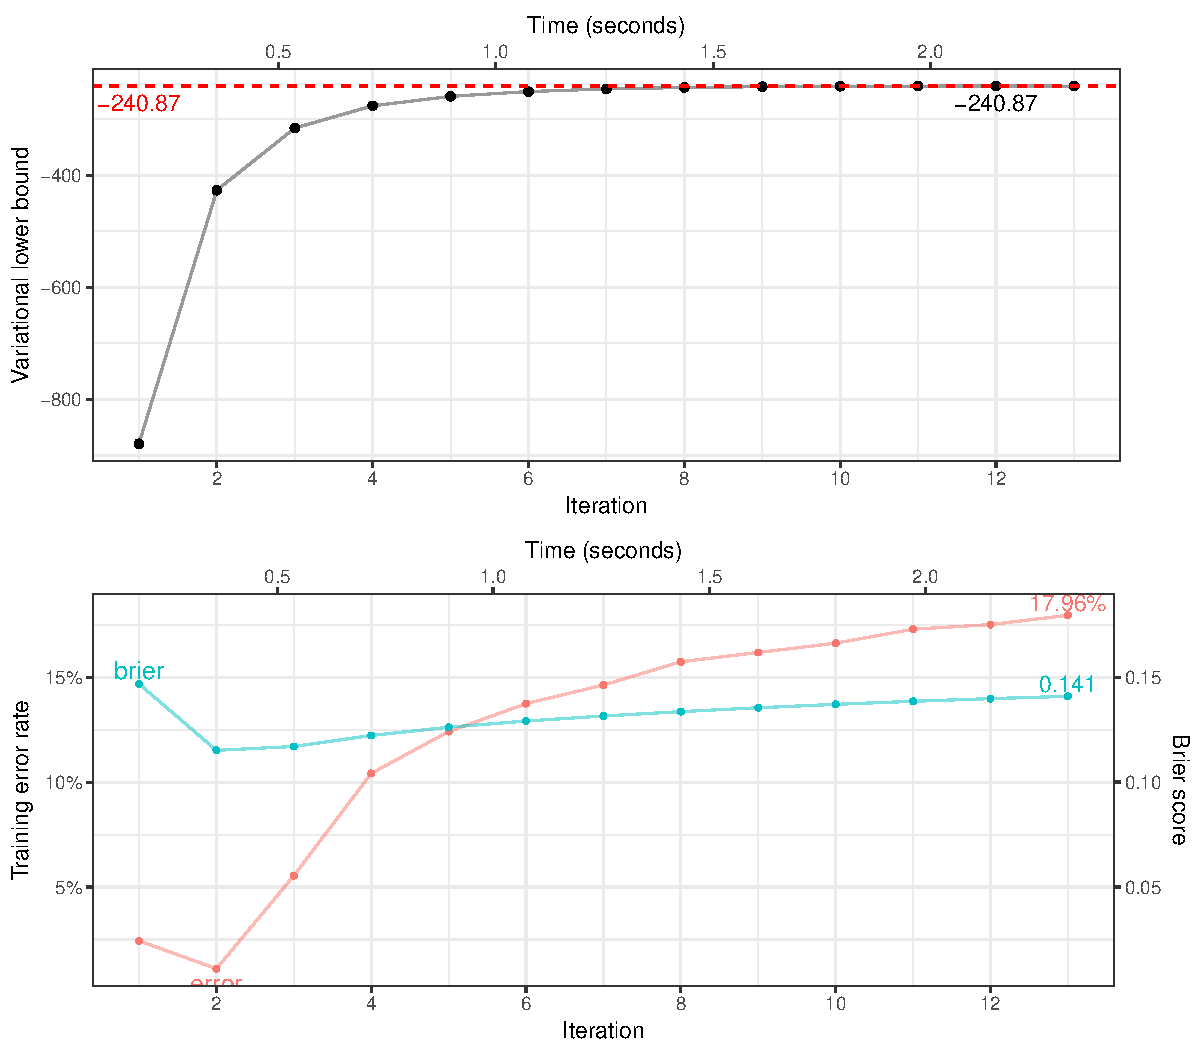
\includegraphics[width=\linewidth]{figure/cardiac_mod_full_plot-1} 

}

\caption[(a) Plot of variational lower bound over time]{(a) Plot of variational lower bound over time. (b) Plot of training error rate and Brier scores over time.}\label{fig:cardiac.mod.full.plot}
\end{figure}


\end{knitrout}

To measure predictive ability, we fit the I-probit model with the canonical and fBm-0.5 kernel on a random subset of the data and obtain the out-of-sample test error rates from the remaining observations. We then compare the results against popular machine learning classifiers, namely: 1) $k$-nearest neighbours; 2) support vector machine; 3) Gaussian process classification (radial basis kernel); 4) random forests; 5) nearest shrunken centroids (Tibshirani et. al. 2003); and 6) L-1 penalised logistic regression. The final model also performs variable selection, something that the I-probit model can do as well, but for now we concentrate on using all the available predictors for training and testing. The experiment is set up as follows:
\begin{enumerate}
  \item Form a training set by sub-sampling $n \in \{50, 100, 200\}$ observations.
  \item The remaining unsampled data is used as the test set.
  \item Fit model on training set, and obtain test error rates defined as
  \[
    \text{test error rate} = \frac{1}{n} \sum_{i=1}^n [y^{\text{pred}}_i \neq y^{\text{test}}_i] \times 100 \%.
  \]
  \item Repeat steps 1-3 100 times to obtain the \emph{average} test error rates and standard errors.
\end{enumerate}
Results for the six methods listed above were obtained from Cannings and Samworth (2017). The results are shown in the plot below.


\begin{knitrout}
\definecolor{shadecolor}{rgb}{1, 1, 1}\color{fgcolor}\begin{figure}

{\centering 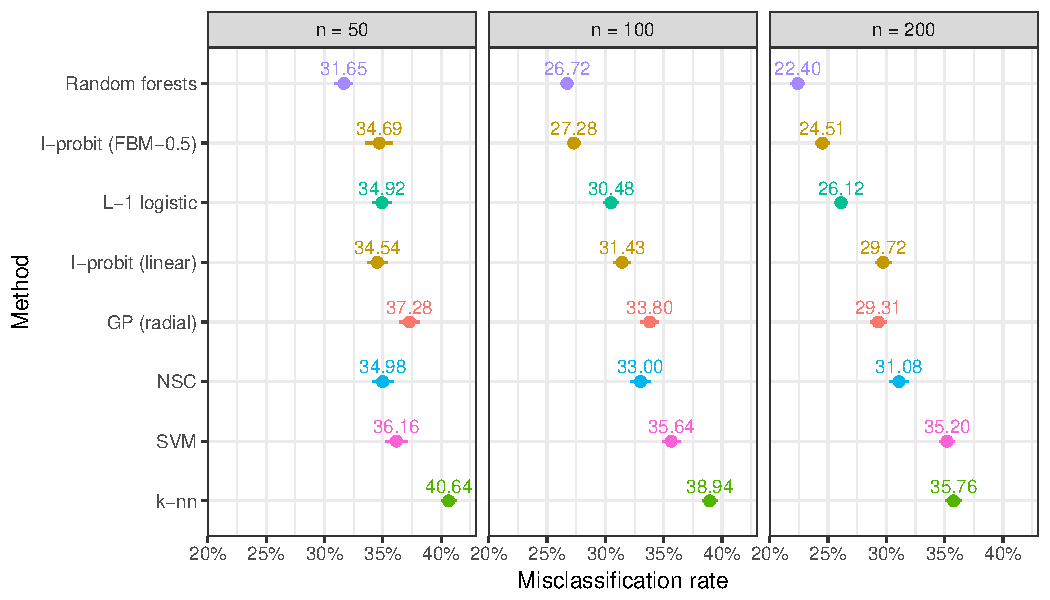
\includegraphics[width=\maxwidth]{figure/plot_cardiac-1} 

}

\caption[Plot of mean test error rates (points) together with the 95\% confidence intervals for I-probit models and six popular classifiers]{Plot of mean test error rates (points) together with the 95\% confidence intervals for I-probit models and six popular classifiers.}\label{fig:plot_cardiac}
\end{figure}


\end{knitrout}

A plot of the mean test error rates together with the 95\% confidence intervals for all models are shown in Figure \ref{fig:plot_cardiac}. The methods shown in the plot are sorted from the best (top) to the worst (bottom), according to a weighted ranking system which favours better performance in smaller sub-samples. It can be seen that the I-probit models outperform the more popular machine learning algorithms out there including $k$-nearest neighbours, support vector machines and Gaussian process classification. The fBm I-probit model performed better than the canonical linear I-probit model, which is unsurprising. An underlying smooth function to model the latent variables is expected to generalise better than a rigid straight line function. The fBm I-probit model came second only to random forests, an ensemble learning method, which depending on the number of random decisions trees generated simultaneously, might be slow. The time complexity of a random forest algorithm is $O(pqn\log(n))$, where $p$ is the number of variables used for training, $q$ is the number of random decision trees, and $n$ is the number of observations.

\end{document}


